% =============================================================================
% FILE NAME : results_and_discussion.tex
% DEPARTMENT: University of Tuebingen
% AUTOR     : Tom Schammo
% =============================================================================
% CONTENT   : Include for chapter "Results and Discussion"
% =============================================================================


\section{Microphones}

\subsection{Implementation}

Driver support for $I^2S$ and PDM has already been implemented into the PULPissimo HAL \cite[Cha 4.3.7]{rust_pulp}.
Unfortunately, however, the microphones did not work right away for reasons listed below.
Unlike the PDM microphone, the $I^2S$ microphone does not work on the PULPissimo chip, due to a hardware compatibility issue.
The $I^2S$ microphone sends a total of 24 bits, one 18-bit word, and 6 zero bits, but the PULPissimo can only handle 16 bits.
While the PDM microphone is compatible with the PULPissimo chip, the Rust drivers were not mature enough for it to work using Rust.

\subsection{Experiments}

To test the functionality of the microphones I played a \SI{1}{\kilo\hertz} sine wave\footnote{Sine wave audio: \url{https://www.youtube.com/watch?v=3FBijeNg_Gs}},
which I then recorded using the microphone.

\subsubsection{I2S Microphone}

\begin{figure}[H]
    \centering
    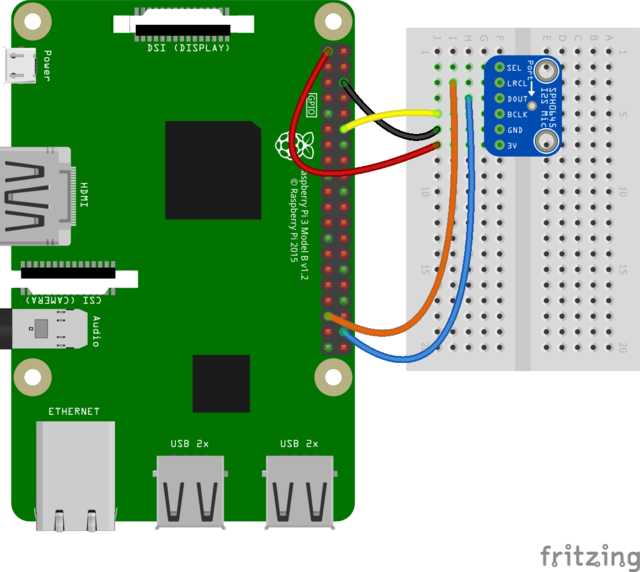
\includegraphics[width=0.5\textwidth]{figures/i2s/wiring_pi.png}
    \caption[$I^2S$ microphone wiring diagram with Raspberry Pi \cite{i2s_wiring}]{$I^2S$ microphone wiring diagram with Raspberry Pi}
    \label{fig:i2s_wiring}
\end{figure}

The $I^2S$ microphone has been wired as displayed in Figure~\ref{fig:i2s_wiring} \cite{i2s_wiring}.
Additionally, SEL has been tied to ground.
The recording was made using this command \lstinline{arecord -D dmic_sv -c2 -r 48000 -f S32_LE -t wav -V mono -v <file name>},
where \emph{<file name>} is the name of the output file.
This creates a 32-bit, PCM-encoded mono WAVE audio file with a sample rate of \SI{48000}{\hertz}.
The \SI{1}{\kilo\hertz} sine wave audio has been played using the speakers of a Redmi Note 7 phone.

\begin{figure}[H]
    \centering
    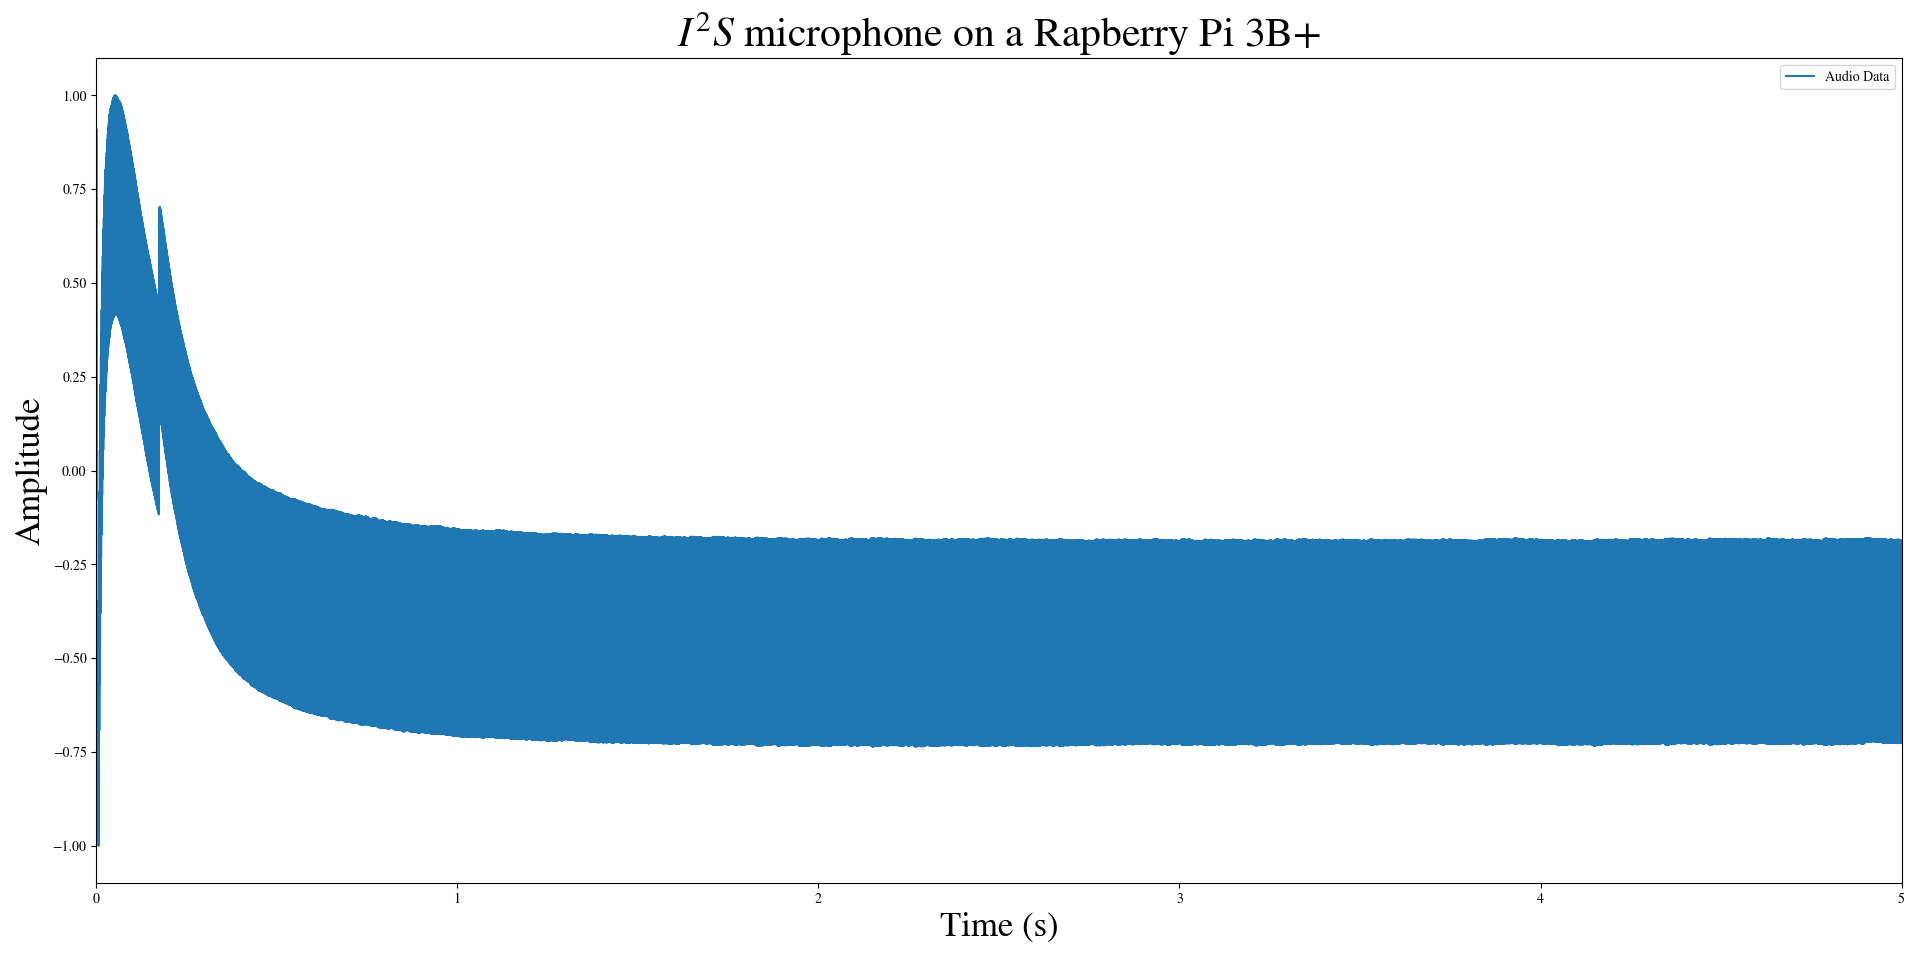
\includegraphics[width=0.9\textwidth]{figures/i2s/i2s_raw_data.png}
    \caption[PCM data of the $I^2S$ microphone plotted]{PCM data of the $I^2S$ microphone plotted}
    \label{fig:i2s_raw}
\end{figure}

When analyzing the raw data displayed in Figure~\ref{fig:i2s_raw}, the spike from seconds 0 to about 0.5
is very noticeable. That is because the microphone seems to have a 'warm-up time', it takes about 1 second for it to be operational and produce clean data.
This has also been noticed on the PULPissimo board with the PDM microphone.
However, after that period, the $I^2S$ microphone is completely operational.
A segment of the recording (normalized) is shown in Figure~\ref{fig:i2s_section}, revealing a clean sine wave.

\begin{figure}[H]
    \centering
    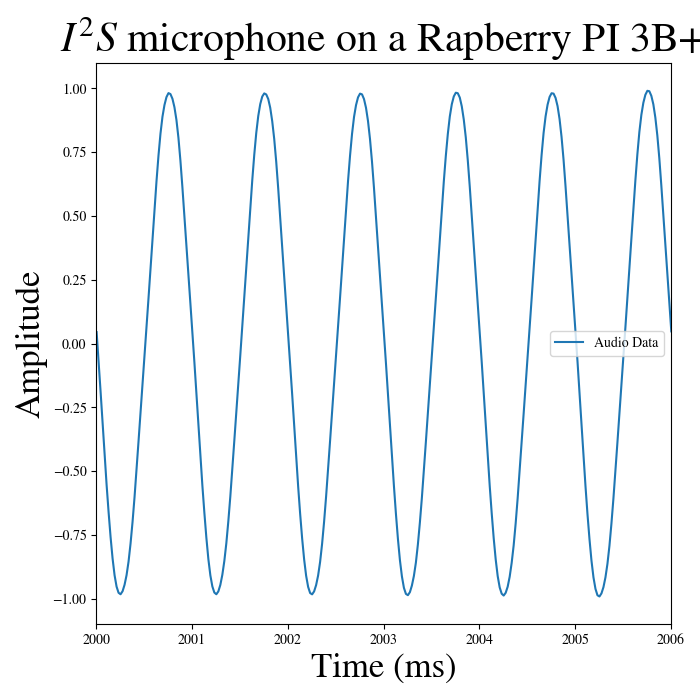
\includegraphics[width=0.9\textwidth]{figures/i2s/i2s_data_recording.png}
    \caption[Sample of normalized PCM data from $I^2S$ microphone]{Sample of normalized PCM data from $I^2S$ microphone}
    \label{fig:i2s_section}
\end{figure}

When taking a close look at a single period and overlaying the data with a perfect sine wave of the same
frequency, displayed in Figure~\ref{fig:i2s_period}, there is a slight, but noticeable discrepancy between the perfect sine
wave and the audio data.
This could have a variety of reasons.
Firstly, the audio that has been played might not have been a perfect sine wave to begin with.
There could've also been variations due to the speakers that had been used, the speakers
might not have produced a 100\% accurate tone.
Or this discrepancy could also be caused by something on the recording side.
Perhaps it is a result of microphone limitations.

\begin{figure}[H]
    \centering
    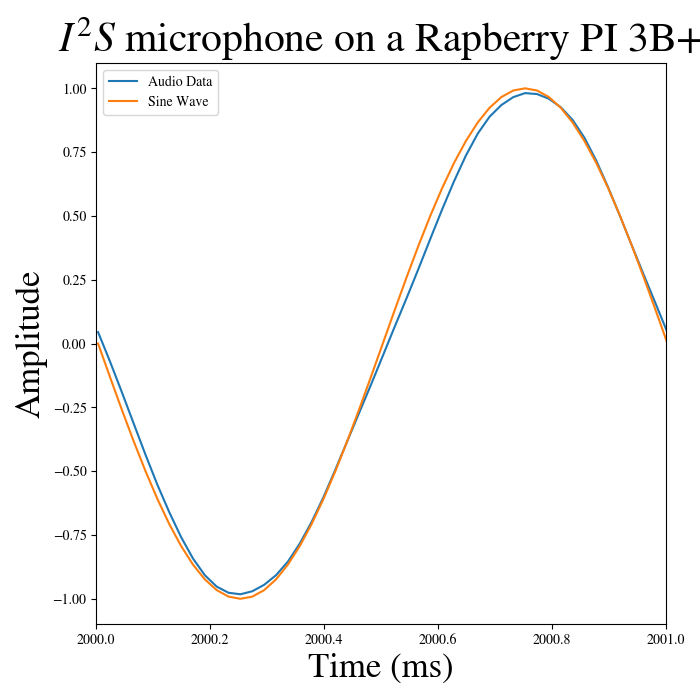
\includegraphics[width=0.9\textwidth]{figures/i2s/i2s_one_period.png}
    \caption[A single period of the normalized audio data, overlaid with a perfect sine wave of the same frequency]{Single period of the audio data, overlaid with sine wave}
    \label{fig:i2s_period}
\end{figure}

\subsubsection{PDM Microphone}

The PDM microphone has been wired as displayed in Figure~\ref{fig:pdm_wiring}.
A logic level converter\footnote{\url{https://cdn-shop.adafruit.com/datasheets/txb0108.pdf}}
has been used because the microphone needs a supply voltage of \SI{3.3}{\volt}, but the
PULPissimo clock uses \SI{1.8}{\volt}.

\begin{figure}[H]
    \centering
    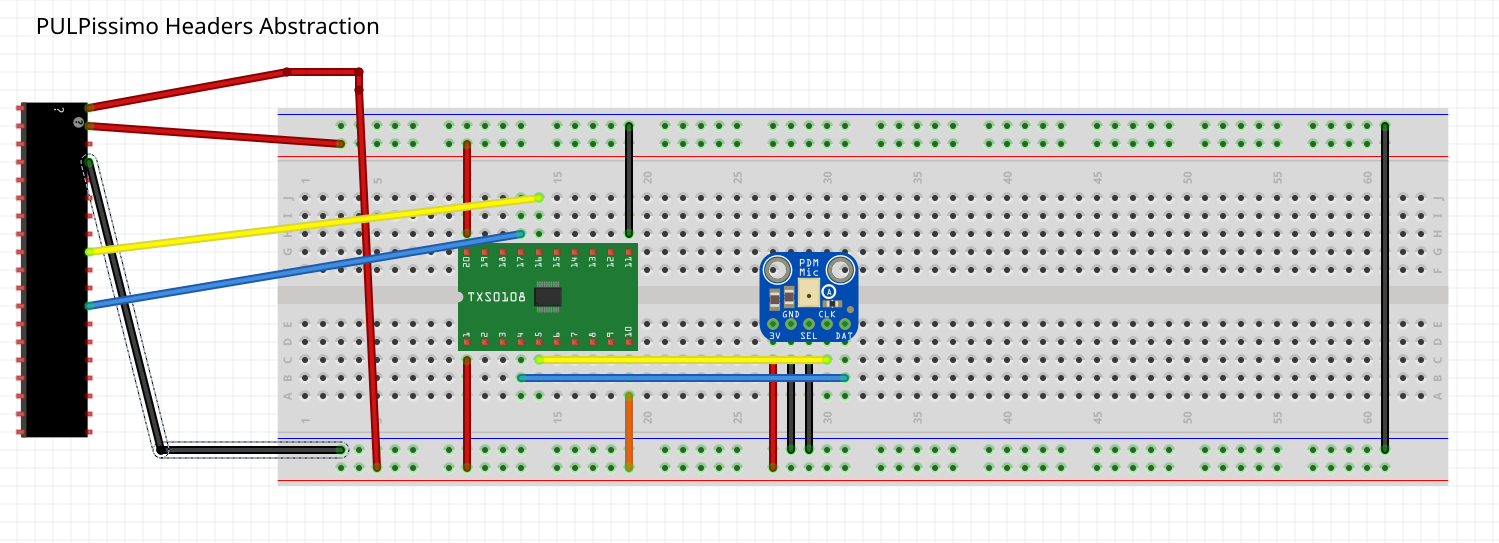
\includegraphics[width=0.9\textwidth]{figures/pdm/wiring.png}
    \caption[PDM microphone wiring with an abstraction for the PULPissimo]{PDM microphone wiring}
    \label{fig:pdm_wiring}
\end{figure}


\begin{figure}[H]
    \centering
    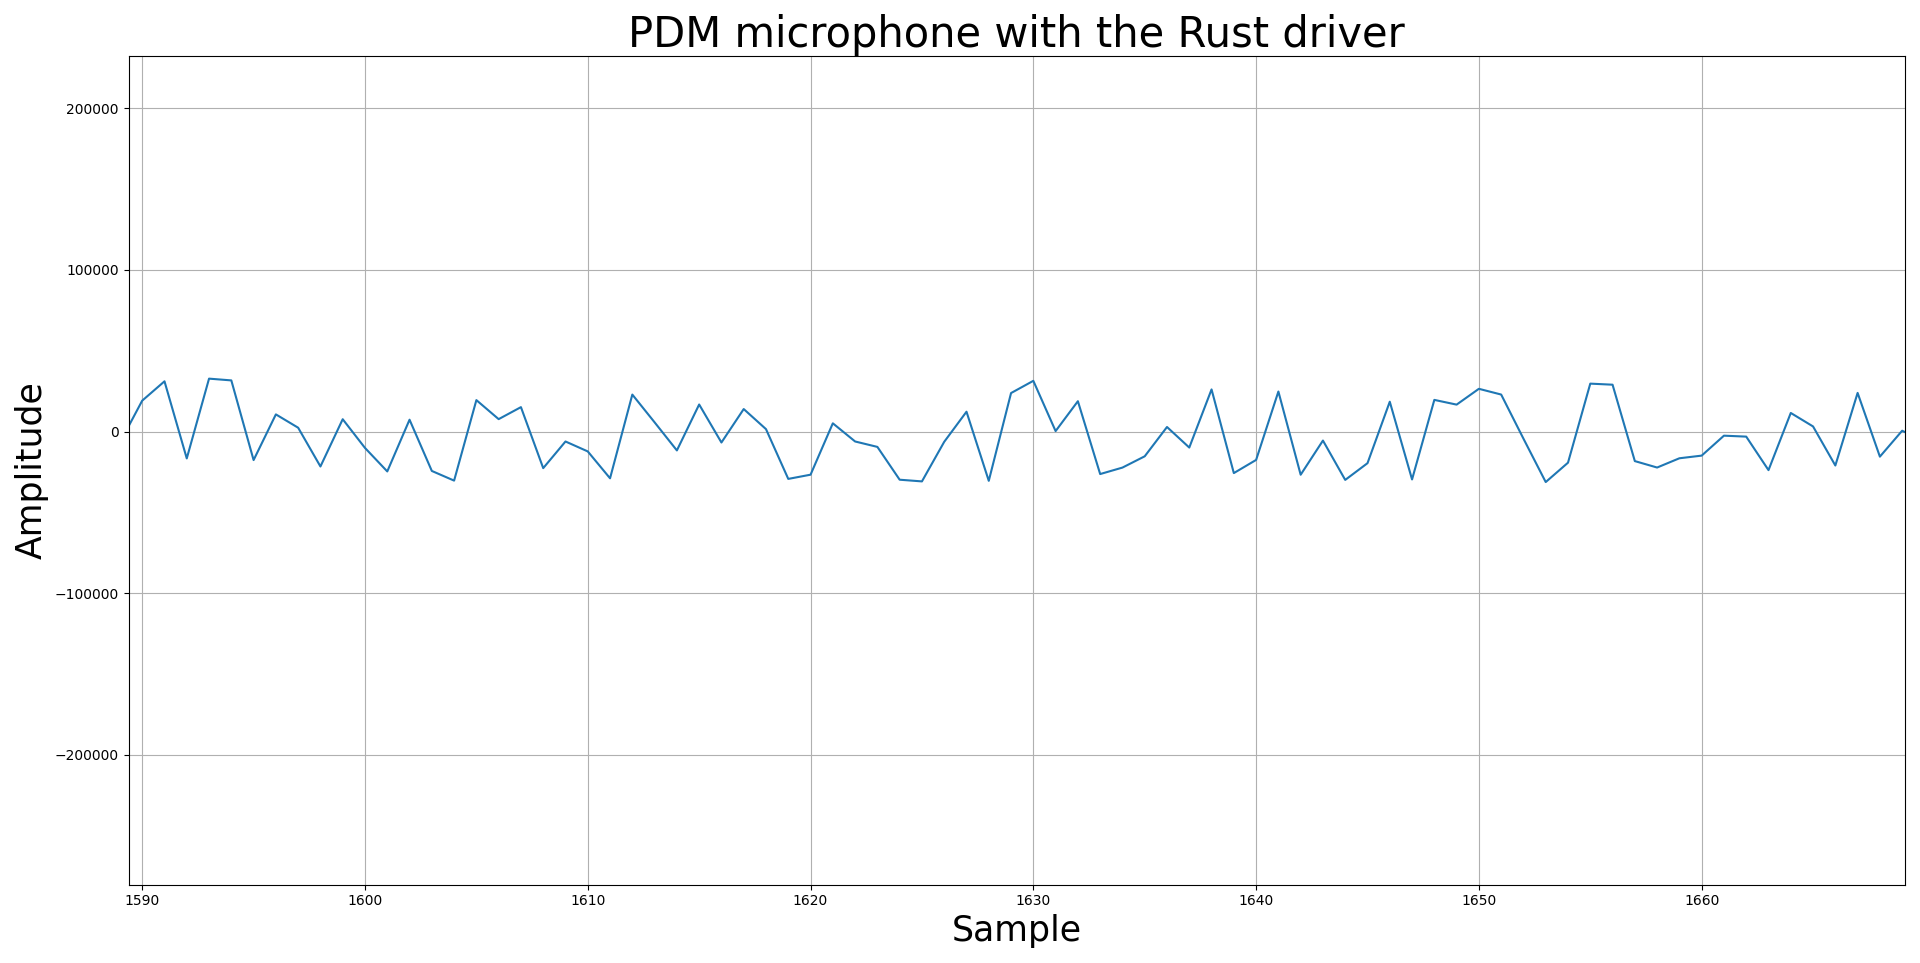
\includegraphics[width=0.9\textwidth]{figures/pdm/pdm_rust.png}
    \caption[Segment of the audio data recorded by the PDM microphone using the Rust driver]{Segment of the audio data recorded by the PDM microphone using the Rust driver}
    \label{fig:pdm_rust}
\end{figure}

Figure~\ref{fig:pdm_rust} shows a section of the recorded PDM data in a PCM encoding, and it is very clear that the driver does not work as intended.
Expected was a sine wave, like in Figure~\ref{fig:pdm_c}, which has been recorded with the same microphone, same wiring using the C driver.

\begin{figure}[H]
    \centering
    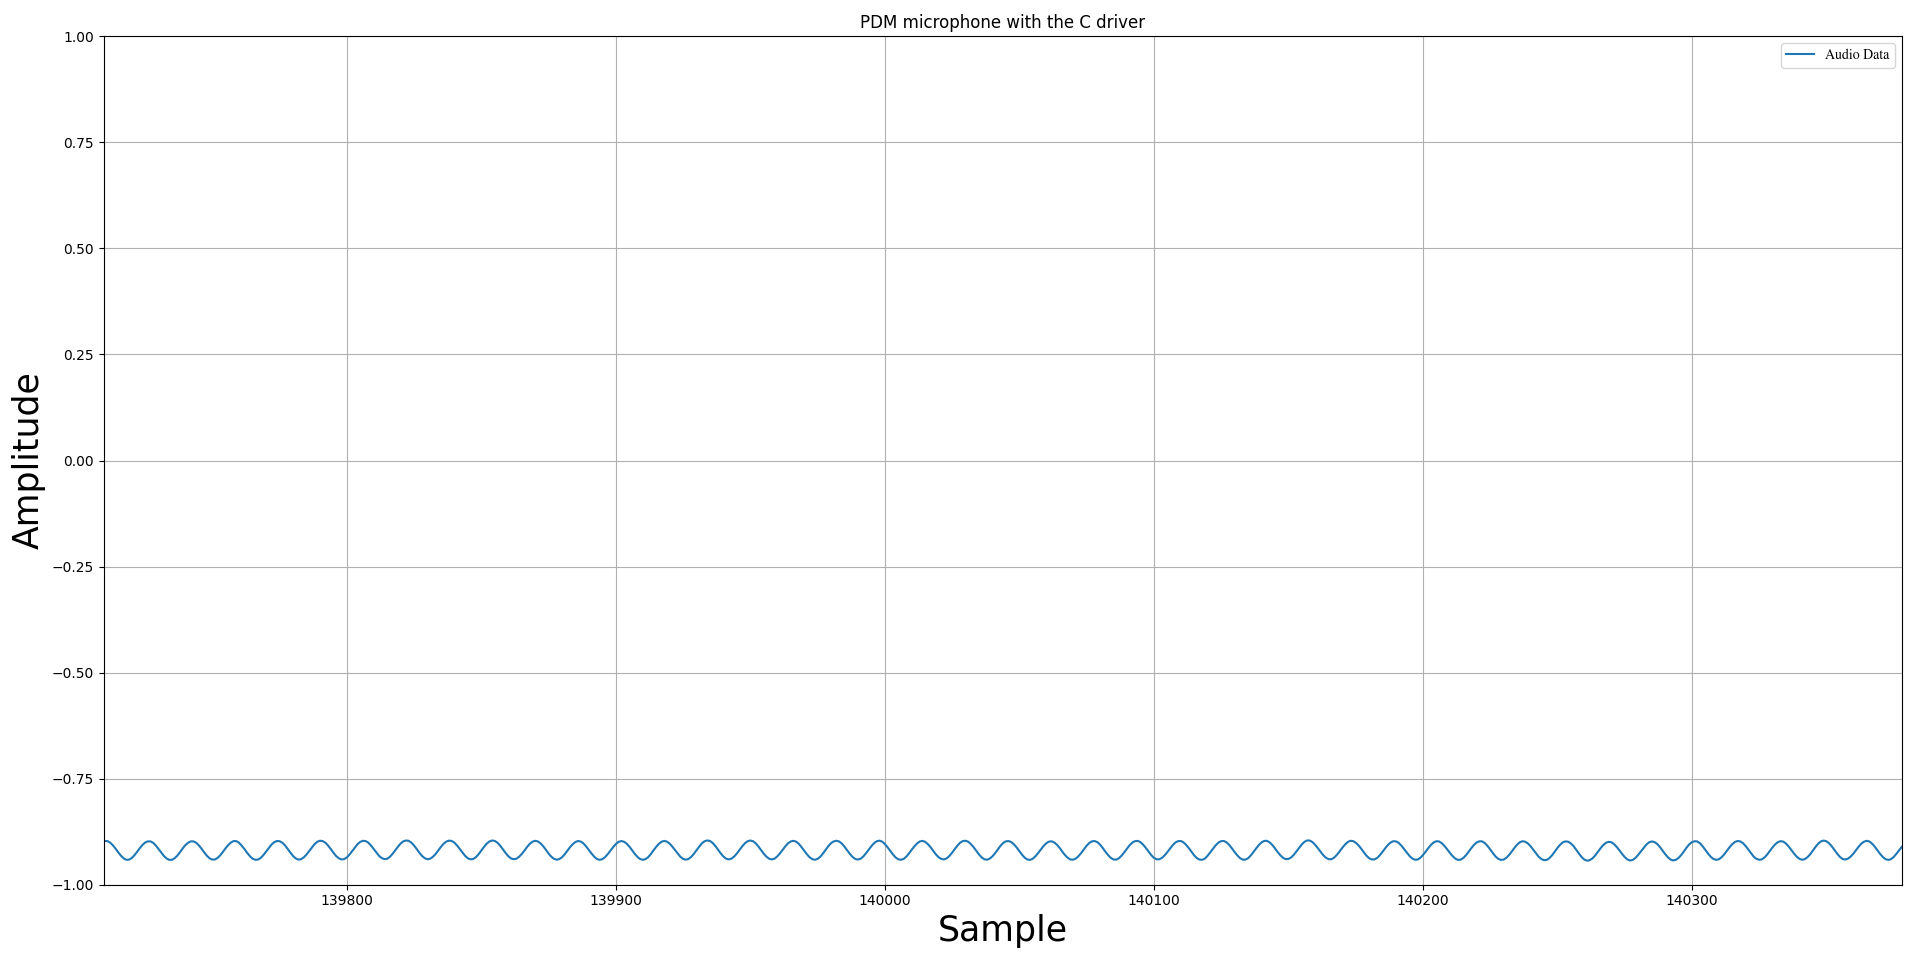
\includegraphics[width=0.9\textwidth]{figures/pdm/pdm_c.png}
    \caption[Segment of the audio data recorded by the PDM microphone using the C driver]{Segment of the audio data recorded by the PDM microphone using the C driver}
    \label{fig:pdm_c}
\end{figure}

\begin{minipage}{\textwidth}
\section{UltraTrail}

\subsection{Implementation}

To implement the driver for UltraTrail, it first has to be added to the SVD file in the PAC
as a peripheral to generate the necessary Rust code to access hardware registers.
Subsequently, the driver can be implemented in the HAL crate.
Finally, I have ported a small program from C to Rust, that contains a set of pre-defined
weights, bias and feature inputs, as well as expected results.
This program can be used to test the implementation of the driver, as it also
performs different configurations by reading and writing the different registers.
\\\\
However, there have been a few differences when it comes to the implementation details.
Most importantly, the C drivers for the PULPissimo provide the \lstinline{__rt_periph_wait_event} function,
which is basically a sophisticated busy wait.
The test code uses that function to wait for UltraTrail to trigger an event interrupt, to announce that
it is done processing as shown in Listing~\ref{code:c_wait_for_event}.
\end{minipage}

\begin{minipage}{\textwidth}
\begin{lstlisting}[style=colorEX,language=C,caption={Waiting for the event in C},label={code:c_wait_for_event}]
pacc_start();

soc_eu_fcEventMask_setEvent(ARCHI_SOC_EVENT_FCHWPE0);
__rt_periph_wait_event(ARCHI_SOC_EVENT_FCHWPE0, 1);

pacc_stop();
\end{lstlisting}
\end{minipage}

However, that function has not been implemented in the Rust drivers, so I had to slightly
vary the implementation of the test code.\\
First I had to define a Mutex \footnote{\url{https://doc.rust-lang.org/std/sync/struct.Mutex.html}}
for the event state, to monitor whether an event interrupt has been triggered as demonstrated
in Listing~\ref{code:mutex}.

\begin{lstlisting}[style=colorEX,language=Rust,caption={Definition of the necessary Mutexes},label={code:mutex}]
static EVENT_STATE: Mutex<Cell<bool>> = Mutex::new(Cell::new(false));
\end{lstlisting}

Subsequently, I defined an event handler as presented in Listing~\ref{code:event_handler}, which
stops the accelerator when it is done and changes the global event state Mutex.

\begin{minipage}{\textwidth}
\begin{lstlisting}[style=colorEX,language=Rust,caption={Event handler function},label={code:event_handler}]
fn hwpe_event_handler() {
    interrupt::free(|cs| {
        unsafe {
            Accelerator::stop_steal();
        }

        EVENT_STATE.borrow(*cs).set(true);
    })
}
\end{lstlisting}
\end{minipage}

After that I just had to enable the event and set the event handler to deal with the event when it is triggered.
The code of that can be seen in Listing~\ref{code:enable_event}.

\begin{minipage}{\textwidth}
\begin{lstlisting}[style=colorEX,language=Rust,caption={Code to enable the hardware event and set the handler},label={code:enable_event}]
unsafe {
    event_interrupt.enable_event(EventId::Hwpe0);
    event_interrupt.set_event_handler(EventId::Hwpe0, hwpe_event_handler);
}
\end{lstlisting}
\end{minipage}

Finally, I could write the busy wait, which basically does nothing until the interrupt is received
and then changes the event state.
An example of that is displayed in Listing~\ref{code:busy_wait}

\begin{minipage}{\textwidth}
\begin{lstlisting}[style=colorEX,language=Rust,caption={Snippet of the busy wait that waits for UltraTrail to finish},label={code:busy_wait}]
accelerator.start();

let mut event = false;
while !event {
    wait_x_nops(1000);

    interrupt::free(|cs| {
        if EVENT_STATE.borrow(*cs).get() {
            event = true;
            EVENT_STATE.borrow(*cs).set(false);
        }
    })
}

// ...
\end{lstlisting}
\end{minipage}

\subsection{Experiments}

The expected results are stored in a vector containing 12 16bit integers, displayed in the Listing~\ref{code:acc_results}.

\begin{minipage}{\textwidth}
\begin{lstlisting}[style=colorEX,language=Rust,caption={The expected results from the driver test},label={code:acc_results}]
let correct_results = [
    0xf246, 0x16bf, 0x08a0, 0xfe52, 0xf709, 0xef58, 0xff6b, 0xf946, 0xfebd, 0x0f40, 0xee45,
    0x18f0,
];
\end{lstlisting}
\end{minipage}

When comparing the code in Listing~\ref{code:acc_results} to the minicom output shown in \ref{code:minicom_out_acc},
one realizes that they match. Which leads me to believe that the UltraTrail driver works as intended.

\begin{minipage}{\textwidth}
\begin{lstlisting}[style=colorEx,caption={Minicom output after executing the driver test},label={code:minicom_out_acc}]
result #0: 0xf246
result #1: 0x16bf
result #2: 0x8a0
result #3: 0xfe52
result #4: 0xf709
result #5: 0xef58
result #6: 0xff6b
result #7: 0xf946
result #8: 0xfebd
result #9: 0xf40
result #10: 0xee45
result #11: 0x18f0
\end{lstlisting}
\end{minipage}
